\documentclass[14pt]{beamer}
\usepackage{./Estilos/BeamerUVM}
\usepackage{./Estilos/ColoresLatex}
%Sección para el tema de beamer, con el theme, usercolortheme y sección de footers
\usetheme{CambridgeUS}
\usecolortheme{default}
%\useoutertheme{default}
\setbeamercovered{invisible}
% or whatever (possibly just delete it)
\setbeamertemplate{section in toc}[sections numbered]
\setbeamertemplate{subsection in toc}[subsections numbered]
\setbeamertemplate{subsection in toc}{\leavevmode\leftskip=3.2em\rlap{\hskip-2em\inserttocsectionnumber.\inserttocsubsectionnumber}\inserttocsubsection\par}
\setbeamercolor{section in toc}{fg=blue}
\setbeamercolor{subsection in toc}{fg=blue}
\setbeamercolor{frametitle}{fg=blue}
\setbeamertemplate{caption}[numbered]

\setbeamertemplate{footline}
\beamertemplatenavigationsymbolsempty
\setbeamertemplate{headline}{}


\makeatletter
\setbeamercolor{secºtion in foot}{bg=gray!30, fg=black!90!orange}
\setbeamercolor{subsection in foot}{bg=blue!30!yellow, fg=red}
\setbeamercolor{date in foot}{bg=black, fg=white}
\setbeamertemplate{footline}
{
  \leavevmode%
  \hbox{%
  \begin{beamercolorbox}[wd=.333333\paperwidth,ht=2.25ex,dp=1ex,center]{section in foot}%
    \usebeamerfont{section in foot} \insertsection
  \end{beamercolorbox}%
  \begin{beamercolorbox}[wd=.333333\paperwidth,ht=2.25ex,dp=1ex,center]{subsection in foot}%
    \usebeamerfont{subsection in foot}  \insertsubsection
  \end{beamercolorbox}%
  \begin{beamercolorbox}[wd=.333333\paperwidth,ht=2.25ex,dp=1ex,right]{date in head/foot}%
    \usebeamerfont{date in head/foot} \insertshortdate{} \hspace*{2em}
    \insertframenumber{} / \inserttotalframenumber \hspace*{2ex} 
  \end{beamercolorbox}}%
  \vskip0pt%
}






% \usefonttheme{serif}
\usepackage[clock]{ifsym}
\usetikzlibrary{plotmarks}
\DeclareSIUnit\erg{erg}
\DeclareSIUnit[number-unit-product = {\,}]\cal{cal}

\sisetup{per-mode=symbol}
\resetcounteronoverlays{saveenumi}

\title{\Large{Práctica 4 - MRU} \\ \normalsize{Física 1}}
\date{7 de julio de 2023}

\begin{document}
\maketitle

\section*{Contenido}
\frame{\frametitle{Contenido} \tableofcontents[currentsection, hideallsubsections]}

\section{La Práctica}
\frame{\tableofcontents[currentsection, hideothersubsections]}
\subsection{Objetivo}

\begin{frame}
\frametitle{Objetivos de la Práctica}
\setbeamercolor{item projected}{bg=bisque,fg=black}
\setbeamertemplate{enumerate items}{%
\usebeamercolor[bg]{item projected}%
\raisebox{1.5pt}{\colorbox{bg}{\color{fg}\footnotesize\insertenumlabel}}%
}
\begin{enumerate}[<+->]
\item Calcular la velocidad de tres corredoras, a partir de un conjunto de datos.
\item Graficar el desplazamiento contra tiempo, de cada corredora.
\end{enumerate}
\end{frame}

\subsection{Actividades}

\begin{frame}
\frametitle{Actividades a realizar}
Se te presentará una tabla con datos de tres corredoras: desplazamiento y tiempo.
\\
\bigskip
\pause
Realiza lo siguiente:
\end{frame}
\begin{frame}
\frametitle{Actividades a realizar}
\setbeamercolor{item projected}{bg=bananayellow,fg=ao}
\setbeamertemplate{enumerate items}{%
\usebeamercolor[bg]{item projected}%
\raisebox{1.5pt}{\colorbox{bg}{\color{fg}\footnotesize\insertenumlabel}}%
}
\begin{enumerate}[<+->]
\item Grafica el desplazamiento contra tiempo, para cada corredora en una misma gráfica.
\item Primero anota una marca $(+, o, *)$, posteriormente dibuja una recta delgada entre cada par de puntos.
\seti
\end{enumerate}
\end{frame}
\begin{frame}
\frametitle{Actividades a realizar}
\setbeamercolor{item projected}{bg=bananayellow,fg=ao}
\setbeamertemplate{enumerate items}{%
\usebeamercolor[bg]{item projected}%
\raisebox{1.5pt}{\colorbox{bg}{\color{fg}\footnotesize\insertenumlabel}}%
}
\begin{enumerate}[<+->]
\conti    
\item En tu cuaderno calcula la velocidad, en cada intervalo de tiempo para las tres corredoras.
\item Grafica la velocidad contra el tiempo para cada corredora, en la misma gráfica.
\end{enumerate}
\end{frame}
\begin{frame}
\frametitle{Los datos a manejar}
\begin{table}
\centering
\small
\renewcommand{\arraystretch}{1}
\begin{tabular}{c | c | c | c }
Distancia [m] & Corredora 1 [s] & Corredora 2 [s] & Corredora 3 [s] \\ \hline
$0$ & $0$ & $0$ & $0$ \\ \hline
$20$ & $1.8$ & $2.6$ & $2.0$ \\ \hline
$50$ & $5.8$ & $6.5$ & $6.0$ \\ \hline
$100$ & $12.0$ & $13.0$ & $12.0$ \\ \hline
$200$ & $25.0$ & $26.0$ & $24.0$ \\ \hline
$300$ & $39.0$ & $39.0$ & $36.0$ \\ \hline
$350$ & $45.0$ & $45.0$ & $42.0$ \\ \hline
$400$ & $51.0$ & $52.0$ & $48.8$ \\ \hline
\end{tabular}
\end{table}
\end{frame}
\begin{frame}
\frametitle{La primera gráfica d vs t}
\begin{figure}
    \centering
    \begin{tikzpicture}[scale=0.8]
        \draw (0, 0) -- (12, 0) node [above, pos=1] {\small{$t \, [s]$}};
        \draw (0, 0) -- (0, 6.3) node [left, pos=1.1] {\small{$d \, [m]$}};

        \node at (-0.6, 0.3) {\footnotesize{$20$}};
        \node at (-0.6, 0.75) {\footnotesize{$50$}};
        \node at (-0.6, 1.5) {\footnotesize{$100$}};
        \node at (-0.6, 6) {\footnotesize{$400$}};
        
        \foreach \y in {0.3, 0.75, 1.5, 6}
            \draw (-0.2, \y) -- (0.2, \y);

        \draw plot[mark=triangle*,mark options={color=blue}, only marks] coordinates {(0, 0)};
        \pause
        \draw (1.8, 0.1) -- (1.8, -0.1);
        \node at (1.8, -0.3) {\scriptsize{$1.8$}};
        \draw plot[mark=triangle*,mark options={color=blue}, only marks] coordinates {(1.8, 0.3)};
        \pause
        \node at (5.8, -0.3) {\scriptsize{$5.8$}};
        \draw (5.8, 0.1) -- (5.8, -0.1);
        \draw plot[mark=triangle*,mark options={color=blue}, only marks] coordinates {(5.8, 0.75)};

        \pause
        \draw [color=blue] (0, 0) -- (1.8, 0.3);

        \pause
        \draw [color=blue] (1.8, 0.3) -- (5.8, 0.75);

        \pause
        \draw (2.6, 0.1) -- (2.6, -0.1);
        \node at (2.6, -0.3) [color=red] {\scriptsize{$2.6$}};
        \draw plot[mark=square*,mark options={color=red}, only marks] coordinates {(2.6, 0.3)};

        \pause
        \draw (6.5, 0.1) -- (6.5, -0.1);
        \node at (6.5, -0.3) [color=red] {\scriptsize{$6.5$}};
        \draw plot[mark=square*,mark options={color=red}, only marks] coordinates {(6.5, 0.75)};

        \pause
        \draw [color=red] (0, 0) -- (2.6, 0.3);

        \pause
        \draw [color=red] (2.6, 0.3) -- (6.5, 0.75);
    \end{tikzpicture}
\end{figure}
\end{frame}
\begin{frame}
\frametitle{Para calcular la velocidad}
Recordemos que para obtener la velocidad, debemos de considerar:
\pause
\begin{eqnarray*}
\begin{aligned}
v = \dfrac{\Delta x}{\Delta t} = \pause \dfrac{x_{f} - x_{i}}{t_{f} - t_{i}}
\end{aligned}
\end{eqnarray*}
Que debemos de realizar para cada intervalo de desplazamiento.
\end{frame}
\begin{frame}
\frametitle{Para calcular la velocidad}
Veamos para la Corredora 1, en el intervalo de $0$ a \SI{20}{\meter}:
\pause
\begin{eqnarray*}
\begin{aligned}
v = \dfrac{x_{f} - x_{i}}{t_{f} - t_{i}} = \pause \dfrac{\SI{20}{\meter} - \SI{0}{\meter}}{\SI{1.8}{\second} - \SI{0}{\second}} = \pause \dfrac{\SI{20}{\meter}}{\SI{1.8}{\second}} = \pause \SI{11.11}{\meter\per\second}
\end{aligned}
\end{eqnarray*}
\end{frame}
\begin{frame}
\frametitle{Para calcular la velocidad}
Para la misma Corredora 1, ahora en el intervalo de \SI{20}{\meter} a \SI{50}{\meter}:
\pause
\begin{eqnarray*}
\begin{aligned}
v = \dfrac{x_{f} - x_{i}}{t_{f} - t_{i}} = \pause \dfrac{\SI{50}{\meter} - \SI{20}{\meter}}{\SI{5.8}{\second} - \SI{1.8}{\second}} = \pause \dfrac{\SI{30}{\meter}}{\SI{4}{\second}} = \pause \SI{7.5}{\meter\per\second}
\end{aligned}
\end{eqnarray*}
\pause
Continuamos calculando la velocidad de la Corredora 1 en cada intervalo de desplazamiento.
\end{frame}
\begin{frame}
\frametitle{Continuamos con las Corredoras 2 y 3}
Hacemos el mismo cálculo de velocidad para las Corredoras 2 y 3, es recomendable hacer una tabla para anotar los valores de la velocidad.
\end{frame}
\begin{frame}
\frametitle{Tabla de velocidades}
\begin{table}
\centering
\small
\renewcommand{\arraystretch}{1}
\begin{tabular}{c | c | c | c }
Intervalo & C1 [m/s] & C2 [m/s] & C3 [m/s] \\ \hline
$0 - 20$ & $11.1$ & & \\ \hline
$20 - 50$ & $7.5$ & & \\ \hline
$50 - 100$ & & & \\ \hline
$100 - 200$ & & & \\ \hline
$200 - 300$ & & & \\ \hline
$300 - 350$ & & & \\ \hline
$350 - 400$ & & & \\ \hline
\end{tabular}
\end{table}
\end{frame}
\begin{frame}
\frametitle{Gráfica de velocidad vs tiempo}
De la tabla anterior, ya podremos graficar las velocidades de cada corredora contra el tiempo.
\\
\bigskip
\pause
Esa gráfica nos servirá para responder las siguientes preguntas.
\end{frame}


\subsection{Preguntas por responder}

\begin{frame}
\frametitle{Preguntas a resolver}
\setbeamercolor{item projected}{bg=red,fg=white}
\setbeamertemplate{enumerate items}{%
\usebeamercolor[bg]{item projected}%
\raisebox{1.5pt}{\colorbox{bg}{\color{fg}\footnotesize\insertenumlabel}}%
}
\begin{enumerate}[<+->]
\item ¿Cuál de las corredoras tiene un mayor cambio de velocidad en el arranque?
\item ¿Quién mantiene durante un mayor tiempo la misma velocidad?
\item ¿Quién aumenta su velocidad al final de la carrera?
\end{enumerate}
\end{frame}

\subsection{El Reporte}

\begin{frame}
\frametitle{El reporte de la Práctica}
El trabajo en el Laboratorio aportará el $80\%$ de la calificación de la Práctica, siempre y cuando se tenga la firma del Profesor en el cuaderno de trabajo.
\\
\bigskip
\pause
Se deberá de agregar una foto con la firma del Profesor en el reporte.
\end{frame}
\begin{frame}
\frametitle{Conclusiones}
Responde las siguientes preguntas:
\setbeamercolor{item projected}{bg=blue,fg=white}
\setbeamertemplate{enumerate items}{%
\usebeamercolor[bg]{item projected}%
\raisebox{1.5pt}{\colorbox{bg}{\color{fg}\footnotesize\insertenumlabel}}%
}
\begin{enumerate}[<+->]
\item ¿Se alcanzaron los objetivos de la Práctica?
\item A partir de una gráfica de desplazamiento vs tiempo, como de velocidad vs tiempo, ¿podrás recuperar la información del movimiento del objeto en estudio?
\item ¿Consideras que esta Práctica es importante en tu formación académica?. Justifica tu respuesta.
\end{enumerate}
\end{frame}
\begin{frame}
\frametitle{Entrega de reporte}
La elaboración y envío del reporte de la Práctica es \textocolor{darkgreen}{INDIVIDUAL}.
\\
\bigskip
\pause
Se abrirá una asignación en Teams para el envío, el plazo vence el próximo martes 11 de julio a las 8 pm.
\end{frame}

\section{La siguiente Práctica}
\frame{\tableofcontents[currentsection, hideothersubsections]}
\subsection{Trabajo Previo}

\begin{frame}
\frametitle{Trabajo para la siguiente práctica}
La siguiente semana abordaremos la Práctica 5 Movimiento Uniformemente Acelerado.
\\
\bigskip
Deberás de resolver el apartado "Investiga y escribe brevemente", que enviarás por asignación en Teams.
\end{frame}
\begin{frame}
\frametitle{Trabajo para la siguiente práctica}
Esto representa $1$ punto de la calificación por Participación.
\\
\bigskip
\pause
El envío se deberá de hacer a más tardar el martes 11 de julio a las 8 pm.
\end{frame}

% \section{Resultados}
% \frame{\tableofcontents[currentsection, hideothersubsections]}
% \subsection{Las gráficas}

% \begin{frame}
% \frametitle{Gráfica de desplazamiento vs tiempo}
% \begin{figure}
%     \centering
%     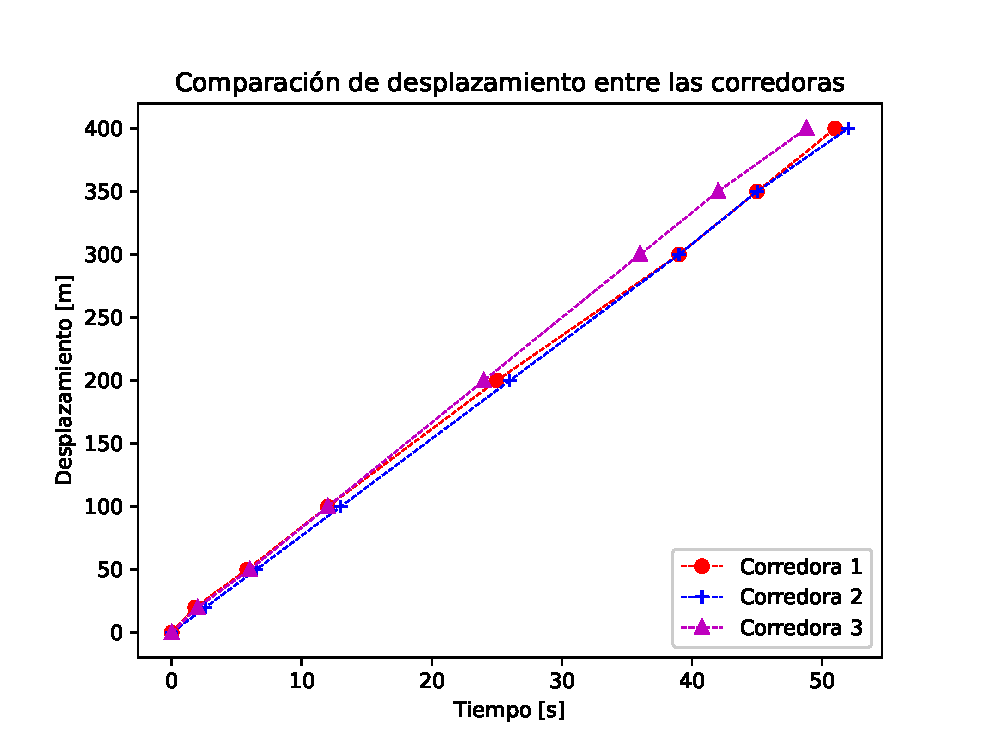
\includegraphics[scale=0.5]{Imagenes/Practica_04_MRU_02.eps}
% \end{figure}
% \end{frame}
% \begin{frame}
% \frametitle{Gráfica de velocidad vs tiempo}
% \begin{figure}
%     \centering
%     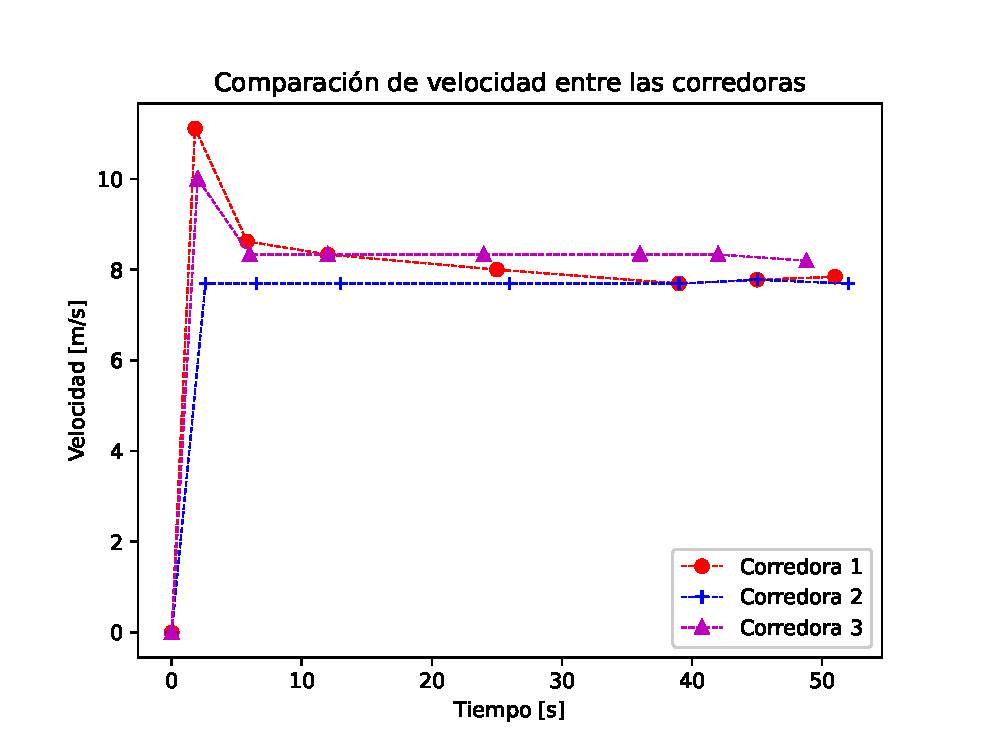
\includegraphics[scale=0.5]{Imagenes/Practica_04_MRU_01.eps}
% \end{figure}
% \end{frame}
\end{document}